\section{Convolution}
In this lecture we are going to deal with the topic of convolution. The general definition is given by:
\[
    (f*g)(x) = \int_{-\infty}^{+\infty} f(t)g(x-t)dt    
\]
The operation can be applied also to vector with:
\[
    (\underline{c}*\underline{d})_K = \sum_{i+j = k} c_i d_j = \sum_i c_i d_{k-i}    
\]
The pedix $K$ is used to indicate the $k$-th element of the vector to which is the convolution is applied. The vectors can be expressed also as polynomials:
\[
    c(x) = c_0 + c_1 x + c_2 x^2 + \dots + c_{n-1} x^{n-1}    
\]
\[
    d(x) = d_0 + d_1 x + d_2 x^2 + \dots + d_{n-1} x^{n-1}
\]
The convolution is the product of these polynomials. [to finish]


\subsection{Cyclic convolution}
The cyclic convolution is a particular case of convolution in which the vectors are cyclic. This means that the last element of the vector is followed by the first one. The cyclic convolution is defined as:
\[
    (\underline{c}\circledast \underline{d})_K = \sum_{i+j = k \mod(n)} c_i d_j 
\]
How can this be written in matrix form?
\begin{multicols}{2}
    \begin{center}
        \textsc{Convolution}
    \end{center}
    In this case are used the \textbf{Toeplitz matrices} (or also called Time-Invariant Linear Systems), the elements are given by $(2n - 1)$-length sequence:
    \[
        \left\{t_K: -(n-1) \leq K \leq (n-1) \right\}    
    \]
    The element in position $(i,j)$ is given by $T(i,j) = t_i - t_j$ and the generic Toeplitz matrix as this shape:
    \[
        T = \begin{bmatrix}
            t_0 & t_{-1} & t_{-2} & \dots & t_{-(n-1)} \\
            t_1 & t_0 & t_{-1} & \dots & t_{-(n-2)} \\
            t_2 & t_1 & t_0 & \dots & t_{-(n-3)} \\
            \vdots & \vdots & \vdots & \ddots & \vdots \\
            t_{n-1} & t_{n-2} & t_{n-3} & \dots & t_0
        \end{bmatrix}    
    \]
    So, it's easy to notice that on the diagonal there is always a constant vector.
    \newcolumn
    \begin{center}
        \textsc{Cyclic convolution}
    \end{center}
    In this case are used the \textbf{Circulant matrices}, a particular case of a Toeplitz matrix. For a given $n \times n$ matrix, the elements are given by $(n)$-length sequence:
    \[
        \left\{c_K: 0 \leq K \leq (n-1) \right\}
    \]
    The element in position $(i,j)$ is given by $C(i,j) = c_{i-j \mod(n)}$ and the generic Circulant matrix as this shape:
    \[
        C = \begin{bmatrix}
            c_0 & c_{n-1} & c_{n-2} & \dots & c_1 \\
            c_1 & c_0 & c_{n-1} & \dots & c_2 \\
            c_2 & c_1 & c_0 & \dots & c_3 \\
            \vdots & \vdots & \vdots & \ddots & \vdots \\
            c_{n-1} & c_{n-2} & c_{n-3} & \dots & c_0
        \end{bmatrix}
    \]
    As you can see, the last element of a column vector becomes the first element of the next column vector, for this reason is called circulant. 
\end{multicols}
Example of circulant matrix:
\[
    C = \begin{bmatrix}
        1 & 8 & 5 & 3\\
        3 & 1 & 8 & 5\\
        5 & 3 & 1 & 8\\
        8 & 5 & 3 & 1
    \end{bmatrix}    
\]
Now we introduce a \textbf{permutation matrix} $P$ defined as follows:
\[
    P = \begin{bmatrix}
        0 & 1 & 0 & 0\\
        0 & 0 & 1 & 0\\
        0 & 0 & 0 & 1\\
        1 & 0 & 0 & 0
    \end{bmatrix}
\]
If we multiply the permutation matrix with a vector, this happen:
\[
    P \underline{c} = \begin{bmatrix}
        0 & 1 & 0 & 0\\
        0 & 0 & 1 & 0\\
        0 & 0 & 0 & 1\\
        1 & 0 & 0 & 0
    \end{bmatrix} \begin{bmatrix}
        c_0\\
        c_1\\
        c_2\\
        c_3
    \end{bmatrix} = \begin{bmatrix}
        c_1\\
        c_2\\
        c_3\\
        c_0
    \end{bmatrix}    
\]
All elements are shifted of 1 position. This means that the circulant matrix $C$ can be built as follows:
\[
    C = c_0 I + c_1 P + c_2 P^2 + c_3 P^3    
\]
This is true for any circulant matrix so we define also $D$:
\[
    D = d_0 I + d_1 P + d_2 P^2 + d_3 P^3 
\]
What happen when we multiply $CD$, i.e two circulant matrices?
\[
    CD = (c_0 I + c_1 P + c_2 P^2 + c_3 P^3)(d_0 I + d_1 P + d_2 P^2 + d_3 P^3)
\]
But this means that we end up with elements with $P^4$ and $P^5$ and so on, but $P^4 = I$, $P^5 = P$ and $P^6 = P^2$. This makes sense even considering that we are dealing with circulant matrices. In general we can say:
\[
    P_n \text{ of } n \times n \implies P^n = I    
\]

\noindent \textbf{Example:}\\
We want to multiply (1,2,1)(3,1,2). We transform the two vectors in two polynomials:
\[
    (1 + 2x + x^2)(3 + x + 2x^2) = 3 + 7x + 7x^2 + 5x^3 + 2x^4    
\]
The terms at the third and forth power must be shifted. 
\[
    (3 + 5) + (7 + 2)x + 7x^2 = 8 + 9x + 7x^2     
\]
The final result is (8,9,7) and, to check its correctness we can consider this sort of property:
\[
    \{(1,2,1) \implies 1+2+1 =4 \times 6 = 3+1+2 \Longleftarrow  (3,1,2) \} \implies 6 \times 4 = 8+9+7 \Longleftarrow  (8,9,7)     
\] 
If we now rename the vectors $\underline{c} = (1,2,1)$ and $\underline{d} = (3,1,2)$, we can compute their convolution by:
\[
    \underline{c} * \underline{d} =     
C\underline{d} = \begin{bmatrix}
        1 & 1 & 2\\
        2 & 1 & 1\\
        1 & 2 & 1
    \end{bmatrix} \begin{bmatrix}
        3\\
        1\\
        2
    \end{bmatrix} = \begin{bmatrix}
        3+1+4\\
        6+1+2\\
        3+2+2
    \end{bmatrix} = \begin{bmatrix}
        8\\
        9\\
        7
    \end{bmatrix}
\]
We have built the circulant matrix starting from the vector $\underline{c}$ and then we have multiplied it with the vector $\underline{d}$. This is the same as multiplying the two polynomials. I did not understand wheter you can either build $C$ from using the initial vector as its row or column.

The matrix $CD$ is circulant because it's the product of two circulant matrices. 

\subsection{Eigenvectors and eigenvalues of a circuland matrix}
Let's start considering again the permutation matrix $P$. We can compute its eigenvalues by using the definition method:
\[
    P - \lambda I = \begin{bmatrix}
        -\lambda & 1 & 0 & 0\\
        0 & -\lambda & 1 & 0\\
        0 & 0 & -\lambda & 1\\
        1 & 0 & 0 & -\lambda
    \end{bmatrix}
    \implies
    \det(P - \lambda I) = \lambda^4 - 1 = 0
\]
\newpage
So the eigenvalues of $P$ are the fourth roots of 1, which correspond to:
\begin{multicols}{2}
    \begin{center}
        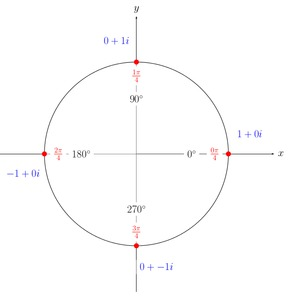
\includegraphics[scale = 0.4]{../images/FourthRoots.jpg}
    \end{center}
    \newcolumn
    \vspace{0.2cm}
    \[
        \begin{split}
            &\lambda^4 - 1 = 0\\
            &\lambda_1 = 1\\
            &\lambda_2 = i\\
            &\lambda_3 = -1\\
            &\lambda_4 = -i
        \end{split}    
    \]
\end{multicols}
We introduce now the complex number $w$ given by:
\[
    w = e^{\dfrac{2\pi i}{n}} \overset{\text{in this case}}{\longrightarrow}    w = e^{\dfrac{2\pi i}{4}} \implies \begin{cases}
        \lambda_1 = w^0\\
        \lambda_2 = w^1\\
        \lambda_3 = w^2\\
        \lambda_4 = w^3
    \end{cases}
\]
In general we have:
\[
    P_n \implies \lambda^n - 1 = 0 \implies w^0, w^1, \dots, w^{n-1}
\]
Another property of $P$: it's orthogonal indeed $P^\intercal P = I$.
What about the eigenvectors of $P$? Consider the generic matrix $C$ written in terms of $P$:
\[
    C = c_0 I + c_1 P + c_2 P^2 + c_3 P^3    
\]
We want to find the eigenvectors of $C$. If $\lambda_k, \underline{v}_k$ is the couple of eigenvalue and eigenvector of $C$, then:
\[
    \begin{split}
        C\underline{v}_k &= \lambda_k \underline{v}_k\\
        (c_0 I + c_1 P + c_2 P^2 + c_3 P^3)\underline{v}_k &= (c_0 + c_1 \lambda_k + c_2 \lambda_k^2 + c_3 \lambda_k^3)\underline{v}_k\\
    \end{split}
\]
$\underline{v}_k$ is an eigenvector of $P$.\\

\noindent \textbf{Example:}\\
\begin{multicols}{4}
    \[
        \begin{split}
            \lambda_1 &= 1\\
            \underline{v}_1 &= \begin{bmatrix}
                1\\
                1\\
                1\\
                1
            \end{bmatrix}    
        \end{split} 
    \]
    \[
        \begin{split}
            \lambda_2 &= i\\
            \underline{v}_2 &= \begin{bmatrix}
                1\\
                i\\
                i^2\\
                i^3
            \end{bmatrix}    
        \end{split} 
    \]
    \[
        \begin{split}
            \lambda_3 &= -1\\
            \underline{v}_3 &= \begin{bmatrix}
                -1\\
                1\\
                -1\\
                1
            \end{bmatrix}    
        \end{split} 
    \]
    \[
        \begin{split}
            \lambda_4 &= -i\\
            \underline{v}_4 &= \begin{bmatrix}
                1\\
                (-i)\\
                (-i)^2\\
                (-i)^3
            \end{bmatrix}    
        \end{split} 
    \]
\end{multicols}    
Example of computation of the third eigenvector:
\[
    \underline{v}_3 = 
    \underbrace{
    \begin{bmatrix}
        0 & 1 & 0 & 0\\
        0 & 0 & 1 & 0\\
        0 & 0 & 0 & 1\\
        1 & 0 & 0 & 0
    \end{bmatrix}   
    \begin{bmatrix}
        1\\
        -1\\
        1\\
        -1
    \end{bmatrix}}_{\begin{bmatrix}
        -1\\
        1\\
        -1\\
        1\\
    \end{bmatrix}}
    = \underbrace{-1
    \begin{bmatrix}
        1\\
        -1\\
        1\\
        -1
    \end{bmatrix}}_{\begin{bmatrix}
        -1\\
        1\\
        -1\\
        1\\
    \end{bmatrix}}
\]
We define 
\[
    \mathbf{F} = \underbrace{\begin{bmatrix}
        1 & 1 & 1 & 1\\
        1 & w & w^2 & w^3\\
        1 & w^2 & w^4 & w^6\\
        1 & w^3 & w^6 & w^9
    \end{bmatrix}}_{\text{eigenvectors}}    
    \underbrace{\dfrac{1}{\sqrt{n}}}_{\text{normalization}} \hspace{0.3cm} \text{where} \hspace{0.3cm} w = e^{\dfrac{2\pi i}{4}}
\]
If you multiply a vector for $\mathbf{F}$ you get its \textbf{Discrete Fourier Transform (DFT)}.
\[
    \underline{\lambda}_c = \begin{bmatrix}
        \lambda_0(c)\\
        \vdots\\
        \lambda_{K-1}(c)
    \end{bmatrix}    
    = 
    \begin{bmatrix}
        c_0 + c_1 + \dots + c_{n-1}\\
        \vdots\\
        c_0 + c_1w^{n-1} + \dots + c_{n-1}w^{(n-1)(n-1)}
    \end{bmatrix}
    =
    \mathbf{F} \begin{bmatrix}
        \underline{c}_0\\
        \vdots\\
        \underline{c}_{n-1}
    \end{bmatrix}
    = \mathbf{F}\underline{c}
\]
Where $\underline{\lambda}_c$ is the vector containing the eigenvalues of the circulant matrix $C$ and $\underline{c}$ is the vector containing the coefficients of the polynomial $c(x)$.\\

Consider two matrices $A$ and $B$, with some eigenvalues and eigenvectors:
\[
    A\underline{v} = \lambda \underline{v} \hspace{0.5cm} B\underline{v} = \gamma \underline{v}    
\]
then
\[
    AB\underline{v} = \gamma A\underline{v} = \gamma \lambda \underline{v}     
\]
So the eigenvalues of the product is the product of the eigenvalues. Now we are going to exploit this property: consider two circulant matrices $C$ and $D$ built from the vectors $\underline{c}$ and $\underline{d}$:
\begin{itemize}
    \item $CD$ in the first row you have the cyclic convolution of $\underline{c}$ and $\underline{d}$ ($\underline{c} \circledast \underline{d}$)
    \item $\mathbf{F}(\underline{c} \circledast \underline{d})$ is the vector of eigenvalues of $CD$
\end{itemize}
Eigenvalues of $C$: $\lambda(c) = \mathbf{F}\underline{c}$ and eigenvalues of $D$: $\lambda(d) = \mathbf{F}\underline{d}$\\
So the eigenvalues of $CD$ are:
\[
    \lambda(CD) = \lambda(C) \cdot^* \lambda(D)= \mathbf{F}\underline{c} \cdot^* \mathbf{F}\underline{d} = \underline{\lambda}_{CD}
\]
Two ways of computing the eigenvalues:
\[
    \mathbf{F}(\underline{C} \circledast \underline{d}) = \mathbf{F}\underline{c} \cdot^* \mathbf{F}\underline{d}
\]
This is called \textbf{Convolution rule}. Which is the fastest method?
The FFT (Fast Fourier Transform) takes $n\log(n)$ operations for computing the matrix multiplication.
\begin{itemize}
    \item $\mathbf{F}(\underline{C} \circledast \underline{d}) = n^2 n\log(n)$
    \item $\mathbf{F}\underline{c} \cdot^* \mathbf{F}\underline{d} = 2n\log(n) + n$ \hspace{0.3cm }so it's better this one!
\end{itemize}